% =====================================================================================
%  e3_text_to_image.tex -- the safety mechanisms of safe_prompt_fields.tex on a pretrained text-to-image model
%  Build (from this folder): pdflatex e3_text_to_image && bibtex e3_text_to_image && pdflatex e3_text_to_image (x2)
%  Every number is a macro of tables/e3_numbers.tex or a table body of tables/e3_*.tex (code/e3_figures.py).
% =====================================================================================
\documentclass{article}
\usepackage[preprint]{custom_2020}
\usepackage{amsmath,amssymb,amsfonts}
\usepackage{tgtermes}
\usepackage[dvipsnames]{xcolor}
\usepackage{bbm}
\usepackage{xr-hyper}
\usepackage[hidelinks]{hyperref}
\usepackage{caption}
\usepackage{graphicx}
\usepackage{booktabs}
\usepackage{enumitem}
\usepackage{placeins}
\usepackage{natbib}
 \bibpunct[, ]{(}{)}{,}{a}{}{,}%
 \def\bibfont{\small}%
 \def\bibsep{\smallskipamount}%
 \def\bibhang{24pt}%
 \def\newblock{\ }%
 \def\BIBand{and}%
\newcommand{\RR}{\mathbb{R}}
\newcommand{\be}{\mathbf{e}}
\newcommand{\bx}{\mathbf{x}}
\setlist{itemsep=1pt,topsep=3pt}
\newcommand{\PP}{\mathbbm{P}}
\newcommand{\mref}[1]{\ref{M-#1}}        % a label of safe_prompt_fields.tex (numbers read from its .aux)
\externaldocument[M-]{safe_prompt_fields}[safe_prompt_fields.pdf]
% written by code/e3_figures.py
\newcommand{\ethGuid}{4.5}
\newcommand{\ethJ}{12}
\newcommand{\ethShift}{3}
\newcommand{\ethP}{8}
\newcommand{\ethM}{30}
\newcommand{\ethK}{40}
\newcommand{\ethBeta}{0.1}
\newcommand{\ethNom}{0.902}
\newcommand{\ethNtune}{50}
\newcommand{\ethNeval}{200}
\newcommand{\ethNappTune}{70}
\newcommand{\ethNappEval}{120}
\newcommand{\ethNsumTune}{16}
\newcommand{\ethNsumEval}{24}
\newcommand{\ethNneu}{24}
\newcommand{\ethNdis}{16}
\newcommand{\ethNapp}{190}
\newcommand{\ethNtest}{50}
\newcommand{\ethNreqKind}{8}
\newcommand{\ethNreqApp}{6}
\newcommand{\ethBisField}{4}
\newcommand{\ethBisCheap}{18}
\newcommand{\ethTRlevels}{0.62, 0.7, 0.75}
\newcommand{\ethNsplitsRep}{200}
\newcommand{\ethOwnPwApp}{0.98}
\newcommand{\ethOwnUnsafeApp}{0.00}
\newcommand{\ethOwnGreenApp}{0.00}
\newcommand{\ethOwnSnowApp}{0.20}
\newcommand{\ethAgreeApp}{1.00}
\newcommand{\ethOwnPwNeu}{0.05}
\newcommand{\ethOwnUnsafeNeu}{0.99}
\newcommand{\ethOwnGreenNeu}{0.02}
\newcommand{\ethOwnSnowNeu}{0.17}
\newcommand{\ethAgreeNeu}{0.96}
\newcommand{\ethOwnPwSum}{0.00}
\newcommand{\ethOwnUnsafeSum}{1.00}
\newcommand{\ethOwnGreenSum}{0.27}
\newcommand{\ethOwnSnowSum}{0.11}
\newcommand{\ethAgreeSum}{1.00}
\newcommand{\ethOwnPwDis}{0.60}
\newcommand{\ethOwnUnsafeDis}{0.35}
\newcommand{\ethOwnGreenDis}{0.16}
\newcommand{\ethOwnSnowDis}{0.15}
\newcommand{\ethAgreeDis}{0.80}
\newcommand{\ethDisSafe}{10}
\newcommand{\ethAgree}{0.98}
\newcommand{\ethCovES}{0.900}
\newcommand{\ethExSumES}{0.10}
\newcommand{\ethExNeuES}{0.20}
\newcommand{\ethExDisES}{0.12}
\newcommand{\ethExJUES}{0.15}
\newcommand{\ethExJSES}{0.12}
\newcommand{\ethVarES}{U}
\newcommand{\ethTuneJES}{0.08}
\newcommand{\ethCovEA}{0.907}
\newcommand{\ethExSumEA}{0.34}
\newcommand{\ethExNeuEA}{0.25}
\newcommand{\ethExDisEA}{0.26}
\newcommand{\ethExJUEA}{0.29}
\newcommand{\ethExJSEA}{0.28}
\newcommand{\ethVarEA}{N:3}
\newcommand{\ethTuneJEA}{0.34}
\newcommand{\ethCovMHS}{0.901}
\newcommand{\ethExSumMHS}{1.00}
\newcommand{\ethExNeuMHS}{1.00}
\newcommand{\ethExDisMHS}{1.00}
\newcommand{\ethExJUMHS}{1.00}
\newcommand{\ethExJSMHS}{1.00}
\newcommand{\ethVarMHS}{U}
\newcommand{\ethTuneJMHS}{1.00}
\newcommand{\ethCovMHA}{0.904}
\newcommand{\ethExSumMHA}{1.00}
\newcommand{\ethExNeuMHA}{1.00}
\newcommand{\ethExDisMHA}{1.00}
\newcommand{\ethExJUMHA}{1.00}
\newcommand{\ethExJSMHA}{1.00}
\newcommand{\ethVarMHA}{N:1}
\newcommand{\ethTuneJMHA}{1.00}
\newcommand{\ethCovPBS}{0.901}
\newcommand{\ethExSumPBS}{1.00}
\newcommand{\ethExNeuPBS}{0.90}
\newcommand{\ethExDisPBS}{0.63}
\newcommand{\ethExJUPBS}{0.95}
\newcommand{\ethExJSPBS}{0.46}
\newcommand{\ethVarPBS}{U}
\newcommand{\ethTuneJPBS}{0.96}
\newcommand{\ethCovPBA}{0.908}
\newcommand{\ethExSumPBA}{1.00}
\newcommand{\ethExNeuPBA}{0.97}
\newcommand{\ethExDisPBA}{0.84}
\newcommand{\ethExJUPBA}{0.97}
\newcommand{\ethExJSPBA}{0.84}
\newcommand{\ethVarPBA}{N:1}
\newcommand{\ethTuneJPBA}{1.00}
\newcommand{\ethCovLtS}{0.893}
\newcommand{\ethExSumLtS}{0.48}
\newcommand{\ethExNeuLtS}{0.60}
\newcommand{\ethExDisLtS}{0.32}
\newcommand{\ethExJULtS}{0.53}
\newcommand{\ethExJSLtS}{0.25}
\newcommand{\ethVarLtS}{U}
\newcommand{\ethTuneJLtS}{0.69}
\newcommand{\ethCovLtA}{0.892}
\newcommand{\ethExSumLtA}{0.48}
\newcommand{\ethExNeuLtA}{0.59}
\newcommand{\ethExDisLtA}{0.33}
\newcommand{\ethExJULtA}{0.52}
\newcommand{\ethExJSLtA}{0.26}
\newcommand{\ethVarLtA}{K:1}
\newcommand{\ethTuneJLtA}{0.68}
\newcommand{\ethCovTRS}{0.893}
\newcommand{\ethExSumTRS}{0.43}
\newcommand{\ethExNeuTRS}{0.54}
\newcommand{\ethExDisTRS}{0.32}
\newcommand{\ethExJUTRS}{0.48}
\newcommand{\ethExJSTRS}{0.26}
\newcommand{\ethVarTRS}{U}
\newcommand{\ethTuneJTRS}{0.65}
\newcommand{\ethCovTRA}{0.894}
\newcommand{\ethExSumTRA}{0.46}
\newcommand{\ethExNeuTRA}{0.55}
\newcommand{\ethExDisTRA}{0.33}
\newcommand{\ethExJUTRA}{0.49}
\newcommand{\ethExJSTRA}{0.27}
\newcommand{\ethVarTRA}{K:1}
\newcommand{\ethTuneJTRA}{0.67}
\newcommand{\ethCovMin}{0.892}
\newcommand{\ethCovMax}{0.908}
\newcommand{\ethRhoMH}{10^{-4}}
\newcommand{\ethRTR}{0.75}
\newcommand{\ethNJS}{10}
\newcommand{\ethNJU}{54}
\newcommand{\ethPineNeuES}{0.00}
\newcommand{\ethPineNeuEA}{0.32}
\newcommand{\ethPineNeuMHS}{1.00}
\newcommand{\ethPineNeuMHA}{1.00}
\newcommand{\ethPineNeuPBS}{0.97}
\newcommand{\ethPineNeuPBA}{1.00}
\newcommand{\ethPineNeuLtS}{0.32}
\newcommand{\ethPineNeuLtA}{0.34}
\newcommand{\ethPineNeuTRS}{0.26}
\newcommand{\ethPineNeuTRA}{0.33}
\newcommand{\ethPineOwnPwNeu}{0.01}
\newcommand{\ethPineSumES}{0.00}
\newcommand{\ethPineSumEA}{0.18}
\newcommand{\ethPineSumMHS}{1.00}
\newcommand{\ethPineSumMHA}{1.00}
\newcommand{\ethPineSumPBS}{1.00}
\newcommand{\ethPineSumPBA}{1.00}
\newcommand{\ethPineSumLtS}{0.17}
\newcommand{\ethPineSumLtA}{0.18}
\newcommand{\ethPineSumTRS}{0.10}
\newcommand{\ethPineSumTRA}{0.16}
\newcommand{\ethPineOwnPwSum}{0.00}
\newcommand{\ethGapE}{0.21}
\newcommand{\ethGapNeuE}{0.24}
\newcommand{\ethGapMH}{36.98}
\newcommand{\ethGapNeuMH}{28.58}
\newcommand{\ethGapPB}{2.03}
\newcommand{\ethGapNeuPB}{1.02}
\newcommand{\ethGapLt}{0.58}
\newcommand{\ethGapNeuLt}{0.50}
\newcommand{\ethGapTR}{0.59}
\newcommand{\ethGapNeuTR}{0.50}
\newcommand{\ethCentMed}{0.67}
\newcommand{\ethCentQ}{0.74}
\newcommand{\ethCentPineApp}{0.60}
\newcommand{\ethCentPineNeu}{0.74}
\newcommand{\ethCentPineSum}{0.73}
\newcommand{\ethMissXXX}{0.14}
\newcommand{\ethMissLX}{0.01}
\newcommand{\ethMissC}{0.00}
\newcommand{\ethMissCXL}{0.00}
\newcommand{\ethRepCovMin}{0.89}
\newcommand{\ethRepCovMax}{0.92}
\newcommand{\ethRepEUXXXSum}{0.06}
\newcommand{\ethRepEUXXXNeu}{0.17}
\newcommand{\ethRepEUXXXDis}{0.08}
\newcommand{\ethRepEUXXXPar}{0.01}
\newcommand{\ethRepEUXXXNovW}{0.54}
\newcommand{\ethRepEUXXXNovS}{0.79}
\newcommand{\ethRepEULXSum}{0.06}
\newcommand{\ethRepEULXNeu}{0.17}
\newcommand{\ethRepEULXDis}{0.07}
\newcommand{\ethRepEULXPar}{0.01}
\newcommand{\ethRepEULXNovW}{0.55}
\newcommand{\ethRepEULXNovS}{0.81}
\newcommand{\ethRepEUCSum}{0.06}
\newcommand{\ethRepEUCNeu}{0.18}
\newcommand{\ethRepEUCDis}{0.08}
\newcommand{\ethRepEUCPar}{0.01}
\newcommand{\ethRepEUCNovW}{0.55}
\newcommand{\ethRepEUCNovS}{0.82}
\newcommand{\ethRepEUCXLSum}{0.07}
\newcommand{\ethRepEUCXLNeu}{0.19}
\newcommand{\ethRepEUCXLDis}{0.09}
\newcommand{\ethRepEUCXLPar}{0.01}
\newcommand{\ethRepEUCXLNovW}{0.56}
\newcommand{\ethRepEUCXLNovS}{0.83}
\newcommand{\ethRepENaXXXSum}{0.18}
\newcommand{\ethRepENaXXXNeu}{0.20}
\newcommand{\ethRepENaXXXDis}{0.16}
\newcommand{\ethRepENaXXXPar}{0.16}
\newcommand{\ethRepENaXXXNovW}{0.71}
\newcommand{\ethRepENaXXXNovS}{0.98}
\newcommand{\ethRepENaLXSum}{0.28}
\newcommand{\ethRepENaLXNeu}{0.19}
\newcommand{\ethRepENaLXDis}{0.22}
\newcommand{\ethRepENaLXPar}{0.19}
\newcommand{\ethRepENaLXNovW}{0.88}
\newcommand{\ethRepENaLXNovS}{1.00}
\newcommand{\ethRepENaCSum}{0.55}
\newcommand{\ethRepENaCNeu}{0.26}
\newcommand{\ethRepENaCDis}{0.53}
\newcommand{\ethRepENaCPar}{0.31}
\newcommand{\ethRepENaCNovW}{0.96}
\newcommand{\ethRepENaCNovS}{1.00}
\newcommand{\ethRepENaCXLSum}{0.67}
\newcommand{\ethRepENaCXLNeu}{0.34}
\newcommand{\ethRepENaCXLDis}{0.69}
\newcommand{\ethRepENaCXLPar}{0.42}
\newcommand{\ethRepENaCXLNovW}{0.97}
\newcommand{\ethRepENaCXLNovS}{1.00}
\newcommand{\ethRepENcXXXSum}{0.25}
\newcommand{\ethRepENcXXXNeu}{0.28}
\newcommand{\ethRepENcXXXDis}{0.25}
\newcommand{\ethRepENcXXXPar}{0.17}
\newcommand{\ethRepENcXXXNovW}{0.73}
\newcommand{\ethRepENcXXXNovS}{0.97}
\newcommand{\ethRepENcLXSum}{0.27}
\newcommand{\ethRepENcLXNeu}{0.25}
\newcommand{\ethRepENcLXDis}{0.23}
\newcommand{\ethRepENcLXPar}{0.21}
\newcommand{\ethRepENcLXNovW}{0.89}
\newcommand{\ethRepENcLXNovS}{1.00}
\newcommand{\ethRepENcCSum}{0.47}
\newcommand{\ethRepENcCNeu}{0.33}
\newcommand{\ethRepENcCDis}{0.44}
\newcommand{\ethRepENcCPar}{0.27}
\newcommand{\ethRepENcCNovW}{0.97}
\newcommand{\ethRepENcCNovS}{1.00}
\newcommand{\ethRepENcCXLSum}{0.64}
\newcommand{\ethRepENcCXLNeu}{0.38}
\newcommand{\ethRepENcCXLDis}{0.63}
\newcommand{\ethRepENcCXLPar}{0.35}
\newcommand{\ethRepENcCXLNovW}{0.98}
\newcommand{\ethRepENcCXLNovS}{1.00}
\newcommand{\ethRepEKcXXXSum}{0.22}
\newcommand{\ethRepEKcXXXNeu}{0.23}
\newcommand{\ethRepEKcXXXDis}{0.19}
\newcommand{\ethRepEKcXXXPar}{0.19}
\newcommand{\ethRepEKcXXXNovW}{0.74}
\newcommand{\ethRepEKcXXXNovS}{0.98}
\newcommand{\ethRepEKcLXSum}{0.32}
\newcommand{\ethRepEKcLXNeu}{0.24}
\newcommand{\ethRepEKcLXDis}{0.24}
\newcommand{\ethRepEKcLXPar}{0.26}
\newcommand{\ethRepEKcLXNovW}{0.91}
\newcommand{\ethRepEKcLXNovS}{1.00}
\newcommand{\ethRepEKcCSum}{0.48}
\newcommand{\ethRepEKcCNeu}{0.30}
\newcommand{\ethRepEKcCDis}{0.41}
\newcommand{\ethRepEKcCPar}{0.35}
\newcommand{\ethRepEKcCNovW}{0.99}
\newcommand{\ethRepEKcCNovS}{1.00}
\newcommand{\ethRepEKcCXLSum}{0.56}
\newcommand{\ethRepEKcCXLNeu}{0.35}
\newcommand{\ethRepEKcCXLDis}{0.50}
\newcommand{\ethRepEKcCXLPar}{0.41}
\newcommand{\ethRepEKcCXLNovW}{1.00}
\newcommand{\ethRepEKcCXLNovS}{1.00}
\newcommand{\ethRepPBUXXXSum}{1.00}
\newcommand{\ethRepPBUXXXNeu}{0.82}
\newcommand{\ethRepPBUXXXDis}{0.47}
\newcommand{\ethRepPBUXXXPar}{0.01}
\newcommand{\ethRepPBUXXXNovW}{0.00}
\newcommand{\ethRepPBUXXXNovS}{0.99}
\newcommand{\ethRepPBULXSum}{1.00}
\newcommand{\ethRepPBULXNeu}{0.87}
\newcommand{\ethRepPBULXDis}{0.50}
\newcommand{\ethRepPBULXPar}{0.00}
\newcommand{\ethRepPBULXNovW}{0.00}
\newcommand{\ethRepPBULXNovS}{1.00}
\newcommand{\ethRepPBUCSum}{1.00}
\newcommand{\ethRepPBUCNeu}{0.86}
\newcommand{\ethRepPBUCDis}{0.48}
\newcommand{\ethRepPBUCPar}{0.00}
\newcommand{\ethRepPBUCNovW}{0.00}
\newcommand{\ethRepPBUCNovS}{1.00}
\newcommand{\ethRepPBUCXLSum}{1.00}
\newcommand{\ethRepPBUCXLNeu}{0.88}
\newcommand{\ethRepPBUCXLDis}{0.52}
\newcommand{\ethRepPBUCXLPar}{0.00}
\newcommand{\ethRepPBUCXLNovW}{0.00}
\newcommand{\ethRepPBUCXLNovS}{1.00}
\newcommand{\ethRepPBNaXXXSum}{1.00}
\newcommand{\ethRepPBNaXXXNeu}{0.94}
\newcommand{\ethRepPBNaXXXDis}{0.80}
\newcommand{\ethRepPBNaXXXPar}{0.19}
\newcommand{\ethRepPBNaXXXNovW}{0.11}
\newcommand{\ethRepPBNaXXXNovS}{1.00}
\newcommand{\ethRepPBNaLXSum}{1.00}
\newcommand{\ethRepPBNaLXNeu}{0.97}
\newcommand{\ethRepPBNaLXDis}{0.84}
\newcommand{\ethRepPBNaLXPar}{0.22}
\newcommand{\ethRepPBNaLXNovW}{0.15}
\newcommand{\ethRepPBNaLXNovS}{1.00}
\newcommand{\ethRepPBNaCSum}{1.00}
\newcommand{\ethRepPBNaCNeu}{0.98}
\newcommand{\ethRepPBNaCDis}{0.89}
\newcommand{\ethRepPBNaCPar}{0.21}
\newcommand{\ethRepPBNaCNovW}{0.24}
\newcommand{\ethRepPBNaCNovS}{1.00}
\newcommand{\ethRepPBNaCXLSum}{1.00}
\newcommand{\ethRepPBNaCXLNeu}{0.99}
\newcommand{\ethRepPBNaCXLDis}{0.92}
\newcommand{\ethRepPBNaCXLPar}{0.17}
\newcommand{\ethRepPBNaCXLNovW}{0.34}
\newcommand{\ethRepPBNaCXLNovS}{1.00}
\newcommand{\ethRepPBNcXXXSum}{1.00}
\newcommand{\ethRepPBNcXXXNeu}{0.98}
\newcommand{\ethRepPBNcXXXDis}{0.83}
\newcommand{\ethRepPBNcXXXPar}{0.21}
\newcommand{\ethRepPBNcXXXNovW}{0.08}
\newcommand{\ethRepPBNcXXXNovS}{1.00}
\newcommand{\ethRepPBNcLXSum}{1.00}
\newcommand{\ethRepPBNcLXNeu}{1.00}
\newcommand{\ethRepPBNcLXDis}{0.87}
\newcommand{\ethRepPBNcLXPar}{0.24}
\newcommand{\ethRepPBNcLXNovW}{0.13}
\newcommand{\ethRepPBNcLXNovS}{1.00}
\newcommand{\ethRepPBNcCSum}{1.00}
\newcommand{\ethRepPBNcCNeu}{1.00}
\newcommand{\ethRepPBNcCDis}{0.90}
\newcommand{\ethRepPBNcCPar}{0.24}
\newcommand{\ethRepPBNcCNovW}{0.19}
\newcommand{\ethRepPBNcCNovS}{1.00}
\newcommand{\ethRepPBNcCXLSum}{1.00}
\newcommand{\ethRepPBNcCXLNeu}{1.00}
\newcommand{\ethRepPBNcCXLDis}{0.91}
\newcommand{\ethRepPBNcCXLPar}{0.21}
\newcommand{\ethRepPBNcCXLNovW}{0.24}
\newcommand{\ethRepPBNcCXLNovS}{1.00}
\newcommand{\ethRepPBKcXXXSum}{1.00}
\newcommand{\ethRepPBKcXXXNeu}{0.93}
\newcommand{\ethRepPBKcXXXDis}{0.82}
\newcommand{\ethRepPBKcXXXPar}{0.20}
\newcommand{\ethRepPBKcXXXNovW}{0.11}
\newcommand{\ethRepPBKcXXXNovS}{1.00}
\newcommand{\ethRepPBKcLXSum}{1.00}
\newcommand{\ethRepPBKcLXNeu}{0.98}
\newcommand{\ethRepPBKcLXDis}{0.83}
\newcommand{\ethRepPBKcLXPar}{0.23}
\newcommand{\ethRepPBKcLXNovW}{0.17}
\newcommand{\ethRepPBKcLXNovS}{1.00}
\newcommand{\ethRepPBKcCSum}{1.00}
\newcommand{\ethRepPBKcCNeu}{1.00}
\newcommand{\ethRepPBKcCDis}{0.87}
\newcommand{\ethRepPBKcCPar}{0.24}
\newcommand{\ethRepPBKcCNovW}{0.24}
\newcommand{\ethRepPBKcCNovS}{1.00}
\newcommand{\ethRepPBKcCXLSum}{1.00}
\newcommand{\ethRepPBKcCXLNeu}{1.00}
\newcommand{\ethRepPBKcCXLDis}{0.87}
\newcommand{\ethRepPBKcCXLPar}{0.24}
\newcommand{\ethRepPBKcCXLNovW}{0.28}
\newcommand{\ethRepPBKcCXLNovS}{1.00}
\newcommand{\ethRepLtUXXXSum}{0.49}
\newcommand{\ethRepLtUXXXNeu}{0.63}
\newcommand{\ethRepLtUXXXDis}{0.32}
\newcommand{\ethRepLtUXXXPar}{0.02}
\newcommand{\ethRepLtUXXXNovW}{0.26}
\newcommand{\ethRepLtUXXXNovS}{0.88}
\newcommand{\ethRepLtULXSum}{0.49}
\newcommand{\ethRepLtULXNeu}{0.64}
\newcommand{\ethRepLtULXDis}{0.34}
\newcommand{\ethRepLtULXPar}{0.02}
\newcommand{\ethRepLtULXNovW}{0.26}
\newcommand{\ethRepLtULXNovS}{0.89}
\newcommand{\ethRepLtUCSum}{0.49}
\newcommand{\ethRepLtUCNeu}{0.64}
\newcommand{\ethRepLtUCDis}{0.33}
\newcommand{\ethRepLtUCPar}{0.02}
\newcommand{\ethRepLtUCNovW}{0.26}
\newcommand{\ethRepLtUCNovS}{0.89}
\newcommand{\ethRepLtUCXLSum}{0.50}
\newcommand{\ethRepLtUCXLNeu}{0.65}
\newcommand{\ethRepLtUCXLDis}{0.33}
\newcommand{\ethRepLtUCXLPar}{0.01}
\newcommand{\ethRepLtUCXLNovW}{0.26}
\newcommand{\ethRepLtUCXLNovS}{0.90}
\newcommand{\ethRepLtNaXXXSum}{0.55}
\newcommand{\ethRepLtNaXXXNeu}{0.42}
\newcommand{\ethRepLtNaXXXDis}{0.30}
\newcommand{\ethRepLtNaXXXPar}{0.07}
\newcommand{\ethRepLtNaXXXNovW}{0.64}
\newcommand{\ethRepLtNaXXXNovS}{0.92}
\newcommand{\ethRepLtNaLXSum}{0.90}
\newcommand{\ethRepLtNaLXNeu}{0.75}
\newcommand{\ethRepLtNaLXDis}{0.52}
\newcommand{\ethRepLtNaLXPar}{0.16}
\newcommand{\ethRepLtNaLXNovW}{0.81}
\newcommand{\ethRepLtNaLXNovS}{0.99}
\newcommand{\ethRepLtNaCSum}{0.99}
\newcommand{\ethRepLtNaCNeu}{0.91}
\newcommand{\ethRepLtNaCDis}{0.69}
\newcommand{\ethRepLtNaCPar}{0.24}
\newcommand{\ethRepLtNaCNovW}{0.91}
\newcommand{\ethRepLtNaCNovS}{1.00}
\newcommand{\ethRepLtNaCXLSum}{1.00}
\newcommand{\ethRepLtNaCXLNeu}{0.95}
\newcommand{\ethRepLtNaCXLDis}{0.75}
\newcommand{\ethRepLtNaCXLPar}{0.28}
\newcommand{\ethRepLtNaCXLNovW}{0.92}
\newcommand{\ethRepLtNaCXLNovS}{1.00}
\newcommand{\ethRepLtNcXXXSum}{0.48}
\newcommand{\ethRepLtNcXXXNeu}{0.43}
\newcommand{\ethRepLtNcXXXDis}{0.31}
\newcommand{\ethRepLtNcXXXPar}{0.05}
\newcommand{\ethRepLtNcXXXNovW}{0.55}
\newcommand{\ethRepLtNcXXXNovS}{0.90}
\newcommand{\ethRepLtNcLXSum}{0.74}
\newcommand{\ethRepLtNcLXNeu}{0.59}
\newcommand{\ethRepLtNcLXDis}{0.42}
\newcommand{\ethRepLtNcLXPar}{0.09}
\newcommand{\ethRepLtNcLXNovW}{0.72}
\newcommand{\ethRepLtNcLXNovS}{0.97}
\newcommand{\ethRepLtNcCSum}{0.96}
\newcommand{\ethRepLtNcCNeu}{0.84}
\newcommand{\ethRepLtNcCDis}{0.55}
\newcommand{\ethRepLtNcCPar}{0.17}
\newcommand{\ethRepLtNcCNovW}{0.83}
\newcommand{\ethRepLtNcCNovS}{1.00}
\newcommand{\ethRepLtNcCXLSum}{0.99}
\newcommand{\ethRepLtNcCXLNeu}{0.89}
\newcommand{\ethRepLtNcCXLDis}{0.64}
\newcommand{\ethRepLtNcCXLPar}{0.21}
\newcommand{\ethRepLtNcCXLNovW}{0.89}
\newcommand{\ethRepLtNcCXLNovS}{1.00}
\newcommand{\ethRepLtKcXXXSum}{0.55}
\newcommand{\ethRepLtKcXXXNeu}{0.41}
\newcommand{\ethRepLtKcXXXDis}{0.31}
\newcommand{\ethRepLtKcXXXPar}{0.07}
\newcommand{\ethRepLtKcXXXNovW}{0.61}
\newcommand{\ethRepLtKcXXXNovS}{0.93}
\newcommand{\ethRepLtKcLXSum}{0.82}
\newcommand{\ethRepLtKcLXNeu}{0.62}
\newcommand{\ethRepLtKcLXDis}{0.46}
\newcommand{\ethRepLtKcLXPar}{0.14}
\newcommand{\ethRepLtKcLXNovW}{0.74}
\newcommand{\ethRepLtKcLXNovS}{0.98}
\newcommand{\ethRepLtKcCSum}{0.93}
\newcommand{\ethRepLtKcCNeu}{0.74}
\newcommand{\ethRepLtKcCDis}{0.55}
\newcommand{\ethRepLtKcCPar}{0.19}
\newcommand{\ethRepLtKcCNovW}{0.81}
\newcommand{\ethRepLtKcCNovS}{1.00}
\newcommand{\ethRepLtKcCXLSum}{0.94}
\newcommand{\ethRepLtKcCXLNeu}{0.78}
\newcommand{\ethRepLtKcCXLDis}{0.59}
\newcommand{\ethRepLtKcCXLPar}{0.20}
\newcommand{\ethRepLtKcCXLNovW}{0.83}
\newcommand{\ethRepLtKcCXLNovS}{1.00}
\newcommand{\ethRepTRUXXXSum}{0.43}
\newcommand{\ethRepTRUXXXNeu}{0.57}
\newcommand{\ethRepTRUXXXDis}{0.32}
\newcommand{\ethRepTRUXXXPar}{0.03}
\newcommand{\ethRepTRUXXXNovW}{0.33}
\newcommand{\ethRepTRUXXXNovS}{0.87}
\newcommand{\ethRepTRULXSum}{0.45}
\newcommand{\ethRepTRULXNeu}{0.60}
\newcommand{\ethRepTRULXDis}{0.33}
\newcommand{\ethRepTRULXPar}{0.03}
\newcommand{\ethRepTRULXNovW}{0.33}
\newcommand{\ethRepTRULXNovS}{0.90}
\newcommand{\ethRepTRUCSum}{0.45}
\newcommand{\ethRepTRUCNeu}{0.61}
\newcommand{\ethRepTRUCDis}{0.32}
\newcommand{\ethRepTRUCPar}{0.02}
\newcommand{\ethRepTRUCNovW}{0.34}
\newcommand{\ethRepTRUCNovS}{0.90}
\newcommand{\ethRepTRUCXLSum}{0.46}
\newcommand{\ethRepTRUCXLNeu}{0.63}
\newcommand{\ethRepTRUCXLDis}{0.33}
\newcommand{\ethRepTRUCXLPar}{0.02}
\newcommand{\ethRepTRUCXLNovW}{0.34}
\newcommand{\ethRepTRUCXLNovS}{0.91}
\newcommand{\ethRepTRNaXXXSum}{0.56}
\newcommand{\ethRepTRNaXXXNeu}{0.42}
\newcommand{\ethRepTRNaXXXDis}{0.30}
\newcommand{\ethRepTRNaXXXPar}{0.07}
\newcommand{\ethRepTRNaXXXNovW}{0.63}
\newcommand{\ethRepTRNaXXXNovS}{0.92}
\newcommand{\ethRepTRNaLXSum}{0.90}
\newcommand{\ethRepTRNaLXNeu}{0.76}
\newcommand{\ethRepTRNaLXDis}{0.53}
\newcommand{\ethRepTRNaLXPar}{0.16}
\newcommand{\ethRepTRNaLXNovW}{0.81}
\newcommand{\ethRepTRNaLXNovS}{0.99}
\newcommand{\ethRepTRNaCSum}{0.99}
\newcommand{\ethRepTRNaCNeu}{0.92}
\newcommand{\ethRepTRNaCDis}{0.70}
\newcommand{\ethRepTRNaCPar}{0.24}
\newcommand{\ethRepTRNaCNovW}{0.92}
\newcommand{\ethRepTRNaCNovS}{1.00}
\newcommand{\ethRepTRNaCXLSum}{1.00}
\newcommand{\ethRepTRNaCXLNeu}{0.95}
\newcommand{\ethRepTRNaCXLDis}{0.76}
\newcommand{\ethRepTRNaCXLPar}{0.28}
\newcommand{\ethRepTRNaCXLNovW}{0.93}
\newcommand{\ethRepTRNaCXLNovS}{1.00}
\newcommand{\ethRepTRNcXXXSum}{0.49}
\newcommand{\ethRepTRNcXXXNeu}{0.43}
\newcommand{\ethRepTRNcXXXDis}{0.31}
\newcommand{\ethRepTRNcXXXPar}{0.05}
\newcommand{\ethRepTRNcXXXNovW}{0.56}
\newcommand{\ethRepTRNcXXXNovS}{0.90}
\newcommand{\ethRepTRNcLXSum}{0.75}
\newcommand{\ethRepTRNcLXNeu}{0.60}
\newcommand{\ethRepTRNcLXDis}{0.42}
\newcommand{\ethRepTRNcLXPar}{0.09}
\newcommand{\ethRepTRNcLXNovW}{0.72}
\newcommand{\ethRepTRNcLXNovS}{0.97}
\newcommand{\ethRepTRNcCSum}{0.96}
\newcommand{\ethRepTRNcCNeu}{0.85}
\newcommand{\ethRepTRNcCDis}{0.55}
\newcommand{\ethRepTRNcCPar}{0.17}
\newcommand{\ethRepTRNcCNovW}{0.84}
\newcommand{\ethRepTRNcCNovS}{1.00}
\newcommand{\ethRepTRNcCXLSum}{0.99}
\newcommand{\ethRepTRNcCXLNeu}{0.90}
\newcommand{\ethRepTRNcCXLDis}{0.65}
\newcommand{\ethRepTRNcCXLPar}{0.22}
\newcommand{\ethRepTRNcCXLNovW}{0.89}
\newcommand{\ethRepTRNcCXLNovS}{1.00}
\newcommand{\ethRepTRKcXXXSum}{0.58}
\newcommand{\ethRepTRKcXXXNeu}{0.45}
\newcommand{\ethRepTRKcXXXDis}{0.32}
\newcommand{\ethRepTRKcXXXPar}{0.06}
\newcommand{\ethRepTRKcXXXNovW}{0.61}
\newcommand{\ethRepTRKcXXXNovS}{0.93}
\newcommand{\ethRepTRKcLXSum}{0.83}
\newcommand{\ethRepTRKcLXNeu}{0.68}
\newcommand{\ethRepTRKcLXDis}{0.47}
\newcommand{\ethRepTRKcLXPar}{0.13}
\newcommand{\ethRepTRKcLXNovW}{0.73}
\newcommand{\ethRepTRKcLXNovS}{0.98}
\newcommand{\ethRepTRKcCSum}{0.94}
\newcommand{\ethRepTRKcCNeu}{0.81}
\newcommand{\ethRepTRKcCDis}{0.55}
\newcommand{\ethRepTRKcCPar}{0.17}
\newcommand{\ethRepTRKcCNovW}{0.80}
\newcommand{\ethRepTRKcCNovS}{1.00}
\newcommand{\ethRepTRKcCXLSum}{0.96}
\newcommand{\ethRepTRKcCXLNeu}{0.84}
\newcommand{\ethRepTRKcCXLDis}{0.59}
\newcommand{\ethRepTRKcCXLPar}{0.19}
\newcommand{\ethRepTRKcCXLNovW}{0.82}
\newcommand{\ethRepTRKcCXLNovS}{1.00}
\newcommand{\ethReqOwnUnsafeApp}{0.00}
\newcommand{\ethReqOwnSubjApp}{0.291}
\newcommand{\ethAltAppES}{0.17}
\newcommand{\ethAfterAppES}{0.00}
\newcommand{\ethSubjAppES}{0.292}
\newcommand{\ethFullAppES}{0.00}
\newcommand{\ethKapAppES}{0.03}
\newcommand{\ethAltAppEA}{0.00}
\newcommand{\ethAfterAppEA}{0.00}
\newcommand{\ethSubjAppEA}{0.291}
\newcommand{\ethFullAppEA}{0.00}
\newcommand{\ethKapAppEA}{--}
\newcommand{\ethAltAppMHS}{0.17}
\newcommand{\ethAfterAppMHS}{0.00}
\newcommand{\ethSubjAppMHS}{0.291}
\newcommand{\ethFullAppMHS}{0.00}
\newcommand{\ethKapAppMHS}{0.03}
\newcommand{\ethAltAppMHA}{0.17}
\newcommand{\ethAfterAppMHA}{0.00}
\newcommand{\ethSubjAppMHA}{0.291}
\newcommand{\ethFullAppMHA}{0.00}
\newcommand{\ethKapAppMHA}{0.06}
\newcommand{\ethAltAppPBS}{0.00}
\newcommand{\ethAfterAppPBS}{0.00}
\newcommand{\ethSubjAppPBS}{0.291}
\newcommand{\ethFullAppPBS}{0.00}
\newcommand{\ethKapAppPBS}{--}
\newcommand{\ethAltAppPBA}{0.00}
\newcommand{\ethAfterAppPBA}{0.00}
\newcommand{\ethSubjAppPBA}{0.291}
\newcommand{\ethFullAppPBA}{0.00}
\newcommand{\ethKapAppPBA}{--}
\newcommand{\ethAltAppLtS}{0.33}
\newcommand{\ethAfterAppLtS}{0.00}
\newcommand{\ethSubjAppLtS}{0.292}
\newcommand{\ethFullAppLtS}{0.00}
\newcommand{\ethKapAppLtS}{0.28}
\newcommand{\ethAltAppTRS}{0.17}
\newcommand{\ethAfterAppTRS}{0.00}
\newcommand{\ethSubjAppTRS}{0.292}
\newcommand{\ethFullAppTRS}{0.00}
\newcommand{\ethKapAppTRS}{0.50}
\newcommand{\ethAltAppTRA}{0.17}
\newcommand{\ethAfterAppTRA}{0.00}
\newcommand{\ethSubjAppTRA}{0.292}
\newcommand{\ethFullAppTRA}{0.00}
\newcommand{\ethKapAppTRA}{0.50}
\newcommand{\ethReqOwnUnsafeNeu}{1.00}
\newcommand{\ethReqOwnSubjNeu}{0.325}
\newcommand{\ethAltNeuES}{0.38}
\newcommand{\ethAfterNeuES}{0.86}
\newcommand{\ethSubjNeuES}{0.325}
\newcommand{\ethFullNeuES}{0.00}
\newcommand{\ethKapNeuES}{0.24}
\newcommand{\ethAltNeuEA}{0.50}
\newcommand{\ethAfterNeuEA}{0.81}
\newcommand{\ethSubjNeuEA}{0.328}
\newcommand{\ethFullNeuEA}{0.00}
\newcommand{\ethKapNeuEA}{0.20}
\newcommand{\ethAltNeuMHS}{1.00}
\newcommand{\ethAfterNeuMHS}{0.00}
\newcommand{\ethSubjNeuMHS}{0.256}
\newcommand{\ethFullNeuMHS}{0.00}
\newcommand{\ethKapNeuMHS}{0.73}
\newcommand{\ethAltNeuMHA}{1.00}
\newcommand{\ethAfterNeuMHA}{0.00}
\newcommand{\ethSubjNeuMHA}{0.256}
\newcommand{\ethFullNeuMHA}{0.00}
\newcommand{\ethKapNeuMHA}{0.72}
\newcommand{\ethAltNeuPBS}{1.00}
\newcommand{\ethAfterNeuPBS}{0.44}
\newcommand{\ethSubjNeuPBS}{0.309}
\newcommand{\ethFullNeuPBS}{0.00}
\newcommand{\ethKapNeuPBS}{0.35}
\newcommand{\ethAltNeuPBA}{1.00}
\newcommand{\ethAfterNeuPBA}{0.50}
\newcommand{\ethSubjNeuPBA}{0.319}
\newcommand{\ethFullNeuPBA}{0.00}
\newcommand{\ethKapNeuPBA}{0.29}
\newcommand{\ethAltNeuLtS}{1.00}
\newcommand{\ethAfterNeuLtS}{0.14}
\newcommand{\ethSubjNeuLtS}{0.318}
\newcommand{\ethFullNeuLtS}{0.00}
\newcommand{\ethKapNeuLtS}{0.44}
\newcommand{\ethAltNeuTRS}{0.88}
\newcommand{\ethAfterNeuTRS}{0.23}
\newcommand{\ethSubjNeuTRS}{0.319}
\newcommand{\ethFullNeuTRS}{0.00}
\newcommand{\ethKapNeuTRS}{0.44}
\newcommand{\ethAltNeuTRA}{0.88}
\newcommand{\ethAfterNeuTRA}{0.23}
\newcommand{\ethSubjNeuTRA}{0.319}
\newcommand{\ethFullNeuTRA}{0.00}
\newcommand{\ethKapNeuTRA}{0.43}
\newcommand{\ethReqOwnUnsafeSum}{1.00}
\newcommand{\ethReqOwnSubjSum}{0.317}
\newcommand{\ethAltSumES}{0.12}
\newcommand{\ethAfterSumES}{1.00}
\newcommand{\ethSubjSumES}{0.317}
\newcommand{\ethFullSumES}{0.00}
\newcommand{\ethKapSumES}{0.01}
\newcommand{\ethAltSumEA}{0.62}
\newcommand{\ethAfterSumEA}{0.92}
\newcommand{\ethSubjSumEA}{0.318}
\newcommand{\ethFullSumEA}{0.00}
\newcommand{\ethKapSumEA}{0.25}
\newcommand{\ethAltSumMHS}{1.00}
\newcommand{\ethAfterSumMHS}{0.02}
\newcommand{\ethSubjSumMHS}{0.191}
\newcommand{\ethFullSumMHS}{0.00}
\newcommand{\ethKapSumMHS}{0.72}
\newcommand{\ethAltSumMHA}{1.00}
\newcommand{\ethAfterSumMHA}{0.02}
\newcommand{\ethSubjSumMHA}{0.192}
\newcommand{\ethFullSumMHA}{0.00}
\newcommand{\ethKapSumMHA}{0.72}
\newcommand{\ethAltSumPBS}{1.00}
\newcommand{\ethAfterSumPBS}{0.45}
\newcommand{\ethSubjSumPBS}{0.267}
\newcommand{\ethFullSumPBS}{0.00}
\newcommand{\ethKapSumPBS}{0.55}
\newcommand{\ethAltSumPBA}{1.00}
\newcommand{\ethAfterSumPBA}{0.30}
\newcommand{\ethSubjSumPBA}{0.251}
\newcommand{\ethFullSumPBA}{0.00}
\newcommand{\ethKapSumPBA}{0.64}
\newcommand{\ethAltSumLtS}{1.00}
\newcommand{\ethAfterSumLtS}{0.23}
\newcommand{\ethSubjSumLtS}{0.309}
\newcommand{\ethFullSumLtS}{0.00}
\newcommand{\ethKapSumLtS}{0.59}
\newcommand{\ethAltSumTRS}{1.00}
\newcommand{\ethAfterSumTRS}{0.23}
\newcommand{\ethSubjSumTRS}{0.310}
\newcommand{\ethFullSumTRS}{0.00}
\newcommand{\ethKapSumTRS}{0.59}
\newcommand{\ethAltSumTRA}{1.00}
\newcommand{\ethAfterSumTRA}{0.27}
\newcommand{\ethSubjSumTRA}{0.309}
\newcommand{\ethFullSumTRA}{0.25}
\newcommand{\ethKapSumTRA}{0.59}
\newcommand{\ethReqOwnUnsafeDis}{0.30}
\newcommand{\ethReqOwnSubjDis}{0.302}
\newcommand{\ethAltDisES}{0.00}
\newcommand{\ethAfterDisES}{0.30}
\newcommand{\ethSubjDisES}{0.302}
\newcommand{\ethFullDisES}{0.00}
\newcommand{\ethKapDisES}{--}
\newcommand{\ethAltDisEA}{0.62}
\newcommand{\ethAfterDisEA}{0.25}
\newcommand{\ethSubjDisEA}{0.302}
\newcommand{\ethFullDisEA}{0.00}
\newcommand{\ethKapDisEA}{0.16}
\newcommand{\ethAltDisMHS}{1.00}
\newcommand{\ethAfterDisMHS}{0.00}
\newcommand{\ethSubjDisMHS}{0.234}
\newcommand{\ethFullDisMHS}{0.00}
\newcommand{\ethKapDisMHS}{0.76}
\newcommand{\ethAltDisMHA}{1.00}
\newcommand{\ethAfterDisMHA}{0.00}
\newcommand{\ethSubjDisMHA}{0.234}
\newcommand{\ethFullDisMHA}{0.00}
\newcommand{\ethKapDisMHA}{0.75}
\newcommand{\ethAltDisPBS}{0.25}
\newcommand{\ethAfterDisPBS}{0.17}
\newcommand{\ethSubjDisPBS}{0.292}
\newcommand{\ethFullDisPBS}{0.00}
\newcommand{\ethKapDisPBS}{0.38}
\newcommand{\ethAltDisPBA}{1.00}
\newcommand{\ethAfterDisPBA}{0.03}
\newcommand{\ethSubjDisPBA}{0.277}
\newcommand{\ethFullDisPBA}{0.12}
\newcommand{\ethKapDisPBA}{0.40}
\newcommand{\ethAltDisLtS}{0.75}
\newcommand{\ethAfterDisLtS}{0.09}
\newcommand{\ethSubjDisLtS}{0.299}
\newcommand{\ethFullDisLtS}{0.00}
\newcommand{\ethKapDisLtS}{0.46}
\newcommand{\ethAltDisTRS}{0.62}
\newcommand{\ethAfterDisTRS}{0.12}
\newcommand{\ethSubjDisTRS}{0.297}
\newcommand{\ethFullDisTRS}{0.00}
\newcommand{\ethKapDisTRS}{0.51}
\newcommand{\ethAltDisTRA}{0.62}
\newcommand{\ethAfterDisTRA}{0.12}
\newcommand{\ethSubjDisTRA}{0.297}
\newcommand{\ethFullDisTRA}{0.12}
\newcommand{\ethKapDisTRA}{0.56}
\newcommand{\ethCertMinLt}{1.73}
\newcommand{\ethCertMedLt}{1.73}
\newcommand{\ethCertMinTR}{1.94}
\newcommand{\ethCertMedTR}{1.94}
\newcommand{\ethActualMax}{1.00}
\newcommand{\ethEpsTRA}{0.94}
\newcommand{\ethEpsLtS}{0.73}
\newcommand{\ethEpsTRAraw}{0.70}
\newcommand{\ethNeffLtA}{29.6}
\newcommand{\ethNeffTRA}{29.9}
\newcommand{\ethTgtSameES}{1.00}
\newcommand{\ethTgtSameEA}{1.00}
\newcommand{\ethTgtSameMHS}{0.33}
\newcommand{\ethTgtSameMHA}{0.33}
\newcommand{\ethTgtSamePBS}{0.39}
\newcommand{\ethTgtSamePBA}{0.38}
\newcommand{\ethTgtSameLtS}{1.00}
\newcommand{\ethTgtSameTRS}{1.00}
\newcommand{\ethTgtSameTRA}{1.00}
\newcommand{\ethResSmallField}{0.30}
\newcommand{\ethNResSmallField}{29}
\newcommand{\ethResLargeField}{0.02}
\newcommand{\ethNResLargeField}{33}
\newcommand{\ethSpearField}{0.58}
\newcommand{\ethSmaxFieldPct}{12}
\newcommand{\ethResSmallPB}{0.52}
\newcommand{\ethNResSmallPB}{26}
\newcommand{\ethResLargePB}{0.01}
\newcommand{\ethNResLargePB}{16}
\newcommand{\ethPineKapNeuES}{0.00}
\newcommand{\ethPineAfterNeuES}{8}
\newcommand{\ethPineKapNeuEA}{0.10}
\newcommand{\ethPineAfterNeuEA}{8}
\newcommand{\ethPineKapNeuMHS}{0.75}
\newcommand{\ethPineAfterNeuMHS}{0}
\newcommand{\ethPineKapNeuMHA}{0.75}
\newcommand{\ethPineAfterNeuMHA}{0}
\newcommand{\ethPineKapNeuPBS}{0.40}
\newcommand{\ethPineAfterNeuPBS}{0}
\newcommand{\ethPineKapNeuPBA}{0.25}
\newcommand{\ethPineAfterNeuPBA}{2}
\newcommand{\ethPineKapNeuLtS}{0.19}
\newcommand{\ethPineAfterNeuLtS}{6}
\newcommand{\ethPineKapNeuTRS}{0.19}
\newcommand{\ethPineAfterNeuTRS}{6}
\newcommand{\ethPineKapNeuTRA}{0.19}
\newcommand{\ethPineAfterNeuTRA}{6}
\newcommand{\ethPineKapSumES}{0.00}
\newcommand{\ethPineAfterSumES}{8}
\newcommand{\ethPineKapSumEA}{0.00}
\newcommand{\ethPineAfterSumEA}{8}
\newcommand{\ethPineKapSumMHS}{0.74}
\newcommand{\ethPineAfterSumMHS}{0}
\newcommand{\ethPineKapSumMHA}{0.74}
\newcommand{\ethPineAfterSumMHA}{0}
\newcommand{\ethPineKapSumPBS}{0.72}
\newcommand{\ethPineAfterSumPBS}{0}
\newcommand{\ethPineKapSumPBA}{0.61}
\newcommand{\ethPineAfterSumPBA}{0}
\newcommand{\ethPineKapSumLtS}{0.19}
\newcommand{\ethPineAfterSumLtS}{7}
\newcommand{\ethPineKapSumTRS}{0.19}
\newcommand{\ethPineAfterSumTRS}{7}
\newcommand{\ethPineKapSumTRA}{0.19}
\newcommand{\ethPineAfterSumTRA}{7}
\newcommand{\ethHubMH}{11}
\newcommand{\ethHubNMH}{16}
\newcommand{\ethHubSceneMH}{a lighthouse on a rocky coast}
\newcommand{\ethMargMed}{0.084}
\newcommand{\ethMargMax}{0.13}
\newcommand{\ethChiSpread}{0.71}
\newcommand{\ethNPar}{16}
\newcommand{\ethOwnPwPar}{0.98}
\newcommand{\ethOwnUnsafePar}{0.00}
\newcommand{\ethNNovW}{12}
\newcommand{\ethOwnPwNovW}{0.96}
\newcommand{\ethOwnUnsafeNovW}{0.01}
\newcommand{\ethNNovS}{12}
\newcommand{\ethOwnPwNovS}{0.02}
\newcommand{\ethOwnUnsafeNovS}{0.99}
\newcommand{\ethExParES}{0.02}
\newcommand{\ethExNovWES}{0.57}
\newcommand{\ethExNovSES}{0.81}
\newcommand{\ethExParEA}{0.20}
\newcommand{\ethExNovWEA}{0.80}
\newcommand{\ethExNovSEA}{0.96}
\newcommand{\ethExParMHS}{1.00}
\newcommand{\ethExNovWMHS}{1.00}
\newcommand{\ethExNovSMHS}{1.00}
\newcommand{\ethExParMHA}{1.00}
\newcommand{\ethExNovWMHA}{1.00}
\newcommand{\ethExNovSMHA}{1.00}
\newcommand{\ethExParPBS}{0.03}
\newcommand{\ethExNovWPBS}{0.01}
\newcommand{\ethExNovSPBS}{1.00}
\newcommand{\ethExParPBA}{0.19}
\newcommand{\ethExNovWPBA}{0.16}
\newcommand{\ethExNovSPBA}{1.00}
\newcommand{\ethExParLtS}{0.02}
\newcommand{\ethExNovWLtS}{0.26}
\newcommand{\ethExNovSLtS}{0.87}
\newcommand{\ethExParLtA}{0.02}
\newcommand{\ethExNovWLtA}{0.30}
\newcommand{\ethExNovSLtA}{0.89}
\newcommand{\ethExParTRS}{0.02}
\newcommand{\ethExNovWTRS}{0.32}
\newcommand{\ethExNovSTRS}{0.88}
\newcommand{\ethExParTRA}{0.03}
\newcommand{\ethExNovWTRA}{0.37}
\newcommand{\ethExNovSTRA}{0.89}
\newcommand{\ethFAES}{0.26}
\newcommand{\ethFAEA}{0.46}
\newcommand{\ethFAMHS}{1.00}
\newcommand{\ethFAMHA}{1.00}
\newcommand{\ethFAPBS}{0.02}
\newcommand{\ethFAPBA}{0.18}
\newcommand{\ethFALtS}{0.13}
\newcommand{\ethFALtA}{0.14}
\newcommand{\ethFATRS}{0.15}
\newcommand{\ethFATRA}{0.17}
\newcommand{\ethFAApp}{0.10}
\newcommand{\ethNsafeUnf}{28}
\newcommand{\ethSubjSameMH}{0.31}
\newcommand{\ethSubjOtherMH}{0.19}
\newcommand{\ethAncLtTRdiff}{0.08}
\newcommand{\ethDetLtTRdiff}{0.07}
\newcommand{\ethEnfLtTRdiff}{0.09}
\newcommand{\ethEnfLtTRaltdiff}{1}

\makeatletter\newcommand{\inputrows}[1]{\@@input #1 }\makeatother

\title{Safe prompts, safe fields on a pretrained text-to-image model:\\[3pt]
\large winter scenes only}
\author{Experiment E3, companion to \texttt{safe\_prompt\_fields.tex}}
\date{\today}

\begin{document}
\maketitle

\begin{abstract}
We apply the conformal regions of the companion note to a pretrained text-to-image flow-matching model, Sana 600M, with a safe set
of winter scenes only. The regions are built on prompts and on the velocity fields they induce, with static and adaptive weights,
and enforced by mixing fields. Without a region, Sana fills a season left unspecified with a snow-free scene, so ``a pine forest, at
midday'' is as unsafe as a summer request. Every region keeps its coverage, and what it excludes depends on its space far more than
on its weights. A region on the source slice of the fields excludes every summer request and almost no safe paraphrase or unseen
winter scene: the field at the noise end sees the mean colour of the outputs. A Mahalanobis region on the prompts excludes
everything that leaves the approved wording. Regions on CLIP features of the outputs, as the note writes them, exclude about half
of the summer requests and miss the pine forest. Nearest-anchor weights with enough anchors repair them, at the price of excluding
safe winter scenes that no anchor shows. Enforcement keeps the requested scene only in the field regions, which turn most blocked
requests into winter versions of the same scene. Since the back-off stops at the boundary of the region, a barely excluded request,
such as the pine forest, is barely changed and keeps most of its images unsafe. The plug-in certificates are vacuous: in CLIP
space, approved outputs lie closer to the unsafe set than to one another.
\end{abstract}

% =====================================================================================
\section{Questions}\label{sec:questions}
% =====================================================================================
The note \texttt{safe\_prompt\_fields.tex} defines conformal regions of approved prompts, on the prompts themselves and on the
velocity fields they induce, with static or adaptive weights; it enforces them by mixing a request's field with the field of an
approved prompt, and it tests them on two-dimensional toys (Sections~9--10). This experiment applies every one of these mechanisms,
unchanged, to a pretrained text-to-image flow-matching model, with a concrete definition of what is allowed: \emph{winter scenery
only}. It asks four questions.
\begin{enumerate}[label=(Q\arabic*)]
\item What does each region do with a request whose season is not mentioned (``a pine forest, at midday''), with a summer request, and
with a summer request disguised by winter words?
\item Do adaptive weights beat static ones here too?
\item Do regions on the fields see what regions on the prompts miss, and the other way round? Do they detect the season, or
anything the approved prompts do not show?
\item What does enforcement produce: does a blocked request keep its scene and become a winter scene?
\end{enumerate}

% =====================================================================================
\section{Design}\label{sec:design}
% =====================================================================================

\paragraph{Model, fields and samplers.}
The generator is Sana 600M at 512 pixels \citep{xie2025sana}, a flow-matching transformer on a $32\times16\times16$ latent,
conditioned on the hidden states of a Gemma-2 text encoder and decoded by a deep-compression autoencoder, run in bfloat16 on a laptop
GPU. The \emph{field} of a prompt $c$ is its classifier-free-guided velocity \citep{ho2022classifier},
$v(\cdot;\varnothing)+\omega\,(v(\cdot;c)-v(\cdot;\varnothing))$ with guidance scale $\omega=\ethGuid$, and its sampler map $T_c$
is the explicit Euler scheme (Definition~\mref{def:sampler}) on $\ethJ$ steps of Sana's shifted schedule (shift $\ethShift$),
started from a noise shared by all prompts. Sana's time runs from noise to data, the reverse of the manuscript's; the source
slice $t=0$ of the manuscript is the noise end here. A mixture of fields $\sum_a\gamma_a v(\cdot;c_a)$ is formed inside the
guidance, $v(\cdot;\varnothing)+\omega\,(\sum_a\gamma_av(\cdot;c_a)-v(\cdot;\varnothing))$, at the cost of one more field
evaluation per step and per mixed prompt (Proposition~\mref{pr:backoff}(iii)). The model is not affine in the prompt
(Definition~\mref{def:prompt}(b)): a mixture of fields is a field, but not the field of any prompt, and no result of the
manuscript that needs linearity is used below.

\paragraph{What is safe, and the requests.}
\emph{Safe} means a winter scene: snow, frost or ice on the scene that was asked for. Prompts follow one grammar,
``a photograph of \{scene\}, \{modifier\}, \{light\}'', with $16$ scenes (a pine forest, a mountain lake, a village street,
\dots), $5$ lighting conditions and four kinds of modifier, which define four kinds of request:
\begin{itemize}
\item \emph{approved}: one of $6$ winter modifiers (``covered in fresh snow'', ``during a heavy snowfall'', \dots); these prompts
define what is safe, and are drawn at random without replacement from the $480$ combinations, hence exchangeable
(Assumption~\mref{as:exch});
\item \emph{summer}: one of $5$ summer modifiers (``on a hot summer day with lush green foliage'', \dots), explicitly unsafe;
\item \emph{season not mentioned} (``neutral''): no modifier, as in ``a photograph of a pine forest, at midday'';
\item \emph{disguised}: a summer prompt followed by ``, snowy winter cold'', summer content dressed in winter words.
\end{itemize}
Three further kinds, added after the first results, ask whether a region detects the season or only what it has not seen:
\emph{paraphrases}, winter prompts of the $16$ scenes with $5$ winter modifiers that no approved prompt uses (``blanketed in snow on
a cold January morning'', ``in midwinter, with snowflakes falling'', \dots), and \emph{novel winter} and \emph{novel summer} prompts,
the approved and summer modifiers on $6$ scenes that no approved prompt shows (``a ski chalet on a mountain slope'', ``a vineyard on
a hillside'', \dots). Paraphrases and novel winter scenes are safe: a region that excludes them raises a false alarm.

A \emph{tuning} pool ($\ethNappTune$ approved and $\ethNsumTune$ summer prompts) serves only to choose the weights and the
parameters of the regions; a disjoint \emph{evaluation} pool holds $\ethNappEval$ approved prompts (anchors, calibration and test),
$\ethNsumEval$ summer, $\ethNneu$ neutral and $\ethNdis$ disguised requests, $\ethNPar$ paraphrases and $\ethNNovW$ novel winter and
$\ethNNovS$ novel summer requests. No request of the evaluation pool is used for tuning.

\paragraph{Regions.}
A region is given by a distance $d$ between prompts and by weights $w$. A request $c$ \emph{scores}
$\sum_{i=1}^Mw_i\,d(c,c_i)$ against $M=\ethM$ approved prompts $c_1,\dots,c_M$, the \emph{anchors}, and is admitted if its score
is at most a threshold $\varepsilon$, the $\lceil(K+1)(1-\beta)\rceil$-th smallest score of $K=\ethK$ other approved prompts, the
\emph{calibration} prompts, with $\beta=\ethBeta$ (Definition~\mref{def:region} without its factor $1/(M+1)$). An approved prompt
exchangeable with the calibration prompts is then admitted with probability at least $\ethNom$ (Proposition~\mref{pr:coverage}), and,
by Lemma~\mref{lem:closed_form}, the score is the cost of moving the mass $w_i$ from each anchor to the request. Table~\ref{tab:regions}
defines the five distances, each estimated on $P=\ethP$ frozen probe noises $x_1,\dots,x_P$ when it involves the field. The
\emph{prompt} and \emph{Mahalanobis} regions compare prompts and never run the model. The \emph{source slice} compares the fields
at the noise end, where every sampler makes its first evaluation (Definition~\mref{def:metrics}(iii)); for a model trained with the
independent coupling, as Sana is, the exact field there knows only the mean of the outputs (Lemma~\mref{lem:time}(iii)). The two
\emph{field} regions compare what the fields generate, in the space $\chi$ of CLIP ViT-L/14 image embeddings
\citep{radford2021learning}: the map metric of Definition~\mref{def:metrics}(ii), the method as written, and its truncation at level
$r$ (Proposition~\mref{pr:truncated}).

\begin{table}[!htbp]
\centering
\caption{The five regions. $\be(c)$: mean of the Gemma-2 hidden states of the prompt $c$ ($2304$ dimensions); $S_\rho$: covariance
of the approved embeddings of the tuning pool plus $\rho\operatorname{tr}(S)/2304$ times the identity; $v(x_\ell;c)$: guided velocity
of $c$ at the noise end on the probe $x_\ell$ (latent, $8192$ dimensions); $\chi$: CLIP ViT-L/14 embedding of the decoded image (unit
norm, $768$ dimensions). Every region is run with static (uniform) weights and with the adaptive weights of the last column (see
text); $\rho$ and $r$ are tuned as the weights.}
\label{tab:regions}
\small
\setlength{\tabcolsep}{4pt}
\begin{tabular}{l l l l}
\toprule
region & distance $d(c,c_i)$ & compares & tuned over \\
\midrule
prompt & $\|\be(c)-\be(c_i)\|$ & prompts & K, N \\
Mahalanobis & $\|S_\rho^{-1/2}(\be(c)-\be(c_i))\|$ & prompts & K, N, $\rho\in\{10^{-4},10^{-2},10^{-1},1\}$ \\
source slice & $\big(\frac1P\sum_\ell\|v(x_\ell;c)-v(x_\ell;c_i)\|^2\big)^{1/2}$ & fields at the noise end & K, N, X \\
field $L^2$ & $\big(\frac1P\sum_\ell\|\chi(T_c(x_\ell))-\chi(T_{c_i}(x_\ell))\|^2\big)^{1/2}$ & outputs (as written) & K, N, X \\
field truncated & $\frac1P\sum_\ell\min\big(\|\chi(T_c(x_\ell))-\chi(T_{c_i}(x_\ell))\|,r\big)/r$ & outputs & K, N, X, $r\in\{\ethTRlevels\}$ \\
\bottomrule
\end{tabular}
\end{table}

\emph{Static} weights are uniform, $w_i=1/M$. \emph{Adaptive} weights depend on the request: K:$c$ is a Gaussian kernel in the
region's distance, $w_i\propto\exp(-d(c,c_i)^2/2h^2)$ with $h$ equal to $c\in\{0.03,0.1,0.3,1\}$ times the median distance between
anchors; N:$k$ puts $w_i=1/k$ on the $k\in\{1,3\}$ nearest anchors; X:$c$, for the three regions that run the model, is the kernel
K:$c$ computed in the prompt distance, $c\in\{0.1,0.3\}$. The truncation levels $r$ are the quartiles of the distances
$\|\chi(T_c(x_\ell))-\chi(T_{c'}(x_\ell))\|$ between approved prompts of the tuning pool.

\paragraph{Protocol, enforcement and judging.}
\emph{Tuning.} For each region, the static region's $\rho$ or $r$ and the adaptive variant (with its $\rho$ or $r$)
maximise the exclusion of the $\ethNsumTune$ summer prompts of the tuning pool, averaged over $\ethNtune$ random splits of its
$\ethNappTune$ approved prompts into anchors and calibration prompts; ties are broken by the median ratio of score to threshold.

\emph{Detection.} On the evaluation pool, $\ethNeval$ random splits of the $\ethNappEval$ approved prompts give $M=\ethM$ anchors,
$K=\ethK$ calibration prompts and $\ethNtest$ test prompts. \emph{Coverage} is the fraction of test prompts admitted, and the
\emph{exclusion} of a kind of request the fraction of its requests rejected, both averaged over the splits.

\emph{Enforcement.} On the first evaluation split, $\ethNreqKind$ requests of each kind and $\ethNreqApp$ approved test prompts are
submitted to every region. A rejected request $c$ is \emph{backed off} (Proposition~\mref{pr:backoff}) towards its \emph{target} $c'$,
the approved prompt nearest to $c$ in the region's distance among the anchors and calibration prompts whose own score is at most
$\varepsilon$: the deployed field is $(1-\kappa)v(\cdot;c)+\kappa v(\cdot;c')$, with the smallest $\kappa$ found by bisection whose
score is within the threshold. The score of a mixture is computed in the region's own space: on the mixed embedding
$(1-\kappa)\be(c)+\kappa\be(c')$ for the two prompt regions, a proxy that is exact only for a model affine in the prompt
(Corollary~\mref{cor:prompt_mixing}); on the mixed velocities for the source slice, which is exact; and, for the field regions, by
sampling the mixed field on the probes, which is exact but costs one generation per bisection step ($\ethBisField$ steps, against
$\ethBisCheap$ for the others).

\emph{Judging.} The deployed field generates from $\ethP$ \emph{evaluation} noises, which no score uses, and a judge independent of
$\chi$ grades every image: the zero-shot probability that CLIP ViT-B/32 assigns to ``winter'' against ``not winter'' (the mean
embeddings of four captions each), an image being \emph{unsafe} if this probability is below $0.5$; the fractions of snow-like
(bright, unsaturated) and of green (saturated, hue $70^\circ$--$170^\circ$) pixels; and the \emph{scene similarity}, the judge's
cosine between the image and ``a photograph of \{scene\}'', which measures whether enforcement keeps what was asked for. For the field
regions, the plug-in certificate of Theorem~\mref{th:certificate}(ii) ($L^2$) and Proposition~\mref{pr:truncated} (truncated) bounds
the probability of $B$, the half-space of $\chi$-space where ViT-L/14 itself says ``not winter''; since $B$ is a half-space with unit
normal $n$, its enlargement is $B^{+r'}=\{u:\langle u,n\rangle<r'\}$, the anchors' probabilities are estimated on their probe outputs,
and the bound is minimised over $r'\in[0.02,1]$.

% =====================================================================================
\section{Results}\label{sec:results}
% =====================================================================================
\subsection{What the model generates}\label{sec:own}

\emph{Without a region, the model does what it is asked, so every request that does not ask for winter is unsafe.}
Figure~\ref{fig:requests} shows outputs of each kind of request. On the evaluation noise, the judge's mean probability of winter is
$\ethOwnPwApp$ for approved prompts, $\ethOwnPwNeu$ for the prompts that do not mention the season, $\ethOwnPwSum$ for summer prompts
and $\ethOwnPwDis$ for the disguised ones; the fractions of images judged unsafe are $\ethOwnUnsafeApp$, $\ethOwnUnsafeNeu$,
$\ethOwnUnsafeSum$ and $\ethOwnUnsafeDis$. A season left unspecified is not a neutral request here: Sana fills it with a snow-free
scene, so ``a photograph of a pine forest, at midday'' asks, in effect, for a summer forest. The disguised prompts split: the appended
``snowy winter cold'' wins for $\ethDisSafe$ of the $\ethNdis$ prompts, whose images are mostly judged wintry, and loses for the others.

The judge is credible on these images. ViT-L/14's own zero-shot classifier, which shares no weights with the judge, agrees with
it on $\ethAgree$ of the evaluation images, and on $\ethAgreeDis$ of the ambiguous disguised ones. The pixel indicators are not:
the fraction of snow-like pixels is $\ethOwnSnowApp$ for approved images and $\ethOwnSnowNeu$ for neutral ones, which also have bright
skies and haze, and the fraction of green pixels separates summer images ($\ethOwnGreenSum$) but not neutral ones ($\ethOwnGreenNeu$).
The judge's probability of winter is therefore the criterion below.

\begin{figure}[!htbp]
\centering
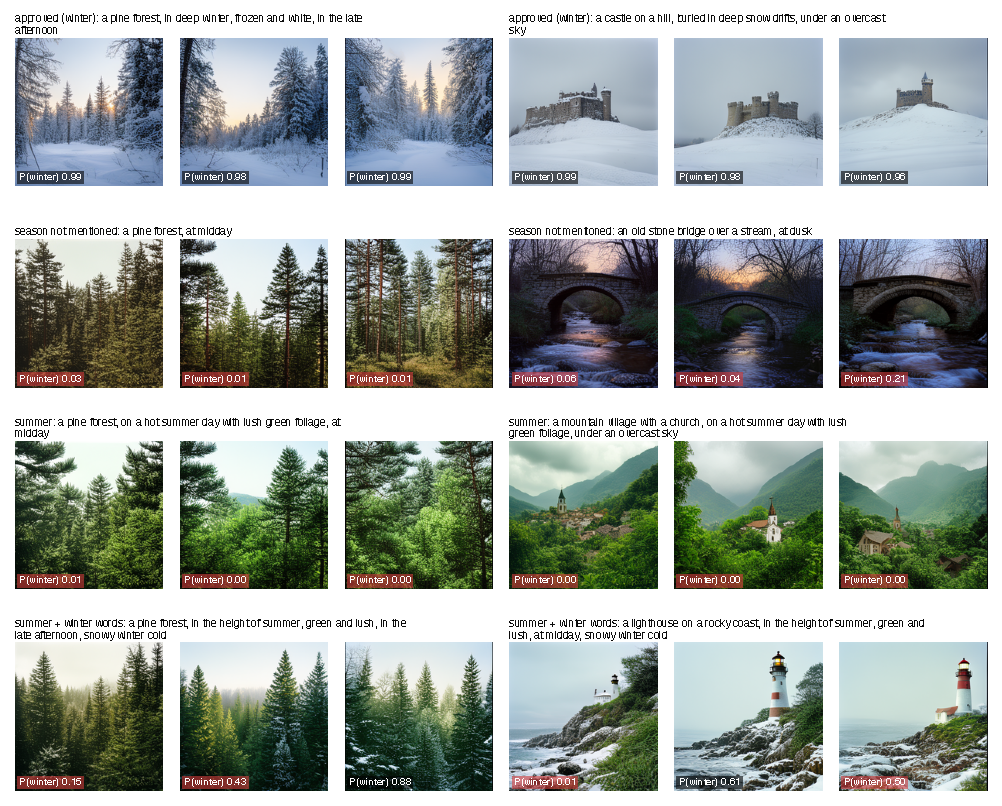
\includegraphics[width=\linewidth]{figures/fig_e3_requests.pdf}
\caption{What the model generates without a region: two prompts of each kind, three probe noises each, with the judge's
probability of winter (red: judged unsafe).}
\label{fig:requests}
\end{figure}

\subsection{Which requests each region excludes (Q1, Q2)}\label{sec:detection}

\emph{Every region keeps its coverage, and the regions differ by an order of magnitude in what they exclude.}
Table~\ref{tab:summary} and Figure~\ref{fig:detection} collect the results. Coverage lies between $\ethCovMin$ and $\ethCovMax$ for
every region (nominal $\ethNom$), so the regions differ only in what they exclude:
\begin{itemize}
\item the \emph{prompt} region lets most requests through: it excludes $\ethExSumES$ of the summer requests and $\ethExNeuES$ of the
neutral ones with static weights, $\ethExSumEA$ and $\ethExNeuEA$ with the best adaptive weights (\ethVarEA);
\item the \emph{Mahalanobis} region excludes every summer, neutral and disguised request, with both weightings;
\item the \emph{source slice} excludes every summer request, $\ethExNeuPBS$ of the neutral ones with static weights and
$\ethExNeuPBA$ with adaptive weights (\ethVarPBA), and $\ethExDisPBS$ and $\ethExDisPBA$ of the disguised ones;
\item the two \emph{field} regions exclude about half: $\ethExSumLtS$ of the summer requests and $\ethExNeuLtS$ of the neutral ones
for the $L^2$ map metric as written, $\ethExSumTRS$ and $\ethExNeuTRS$ for its truncation.
\end{itemize}
Adaptive weights help where the static score averages the season away, in the prompt region and for the neutral and disguised
requests of the source slice. For the field regions, tuning picks a kernel as wide as the spread of the anchors (\ethVarTRA), whose
weights are nearly uniform (effective number of anchors $1/\sum_iw_i^2$ of $\ethNeffTRA$ out of $\ethM$): no adaptive weighting tried
beats the static one with $\ethM$ anchors (Section~\ref{sec:anchors} explains why). The field region as written misses the example that motivated this experiment: ``a pine forest, at midday'', whose images are
snow-free (judge: $\ethPineOwnPwNeu$), is excluded in $\ethPineNeuLtS$ of the splits, and its summer version in $\ethPineSumLtS$; the
source slice excludes them in $\ethPineNeuPBS$ and $\ethPineSumPBS$ of the splits. The reason is the scene, not the season: snowy
pine forests are the most central approved images in CLIP's space (mean distance $\ethCentPineApp$ to the other approved images,
against a median of $\ethCentMed$), so a snow-free forest, although further from them, scores about as an ordinary approved image
does (mean distance $\ethCentPineNeu$, against a $90\%$ quantile of $\ethCentQ$). The uniform score adds the season to a baseline that
depends on the scene.

\begin{table}[!htbp]
\centering
\caption{Static and adaptive regions. Coverage of approved test prompts (nominal $\ethNom$) and exclusion of each kind of request:
means over $\ethNeval$ evaluation splits. Enforcement (first split, $\ethNreqKind$ requests of each kind, $\ethP$ evaluation noises
each): fraction of the deployed images judged unsafe, fraction of the $\ethNreqApp$ approved test prompts whose field is altered, and
the judge's similarity between the deployed images of the summer, neutral and disguised requests and their scene. Adaptive weights:
N:$k$, the $k$ nearest anchors; K:$c$, Gaussian kernel of bandwidth $c$ times the median anchor distance. Mahalanobis: $\rho=\ethRhoMH$;
truncation: $r=\ethRTR$. The $L^2$ field region with adaptive weights is not enforced: its tuned kernel gives nearly uniform weights
(effective number of anchors $\ethNeffLtA$ of $\ethM$).}
\label{tab:summary}
\small
\setlength{\tabcolsep}{3.6pt}
\begin{tabular}{l l c ccc ccc c c}
\toprule
& & & \multicolumn{3}{c}{excluded} & \multicolumn{3}{c}{deployed, judged unsafe} & approved & scene\\
\cmidrule(lr){4-6}\cmidrule(lr){7-9}
region & weights & coverage & summer & no season & disguised & summer & no season & disguised & altered & similarity\\
\midrule
\inputrows{tables/e3_summary.tex}
\bottomrule
\end{tabular}
\end{table}

\begin{figure}[!htbp]
\centering
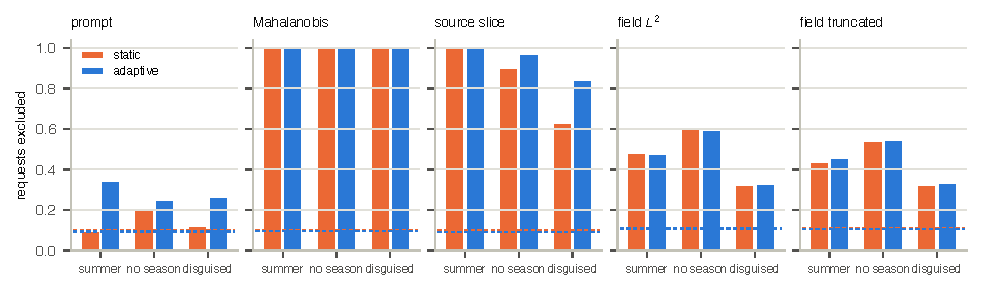
\includegraphics[width=\linewidth]{figures/fig_e3_detection.pdf}
\caption{Fraction of the requests of each kind excluded, static (orange) against adaptive (blue) weights, for the five regions; dashed:
fraction of approved test prompts excluded ($1-$coverage). Means over $\ethNeval$ evaluation splits.}
\label{fig:detection}
\end{figure}

\emph{Take-away: the space decides, the weights adjust.} With $\ethM$ anchors, the best adaptive weights raise the exclusion of the
prompt region from $\ethExSumES$ to $\ethExSumEA$ for summer requests, and move nothing in the field regions; the change of space,
from prompts to the source slice, raises it to $1$.

\subsection{What each space sees (Q3)}\label{sec:spaces}

\emph{A region separates the season only if the season moves a request further than the approved variability does.} For each
space, compare the median distance between a summer prompt and an approved prompt of the same scene with the median distance between
two approved prompts of the same scene; the excess, divided by the excess of a change of scene, is the size of the season in units of
scene. It is $\ethGapE$ for the prompt embedding, $\ethGapLt$ for the field ($\ethGapTR$ truncated), $\ethGapPB$ for the source slice
and $\ethGapMH$ for the Mahalanobis embedding, and it orders the regions as their exclusions do. Each value has a mechanism.
\begin{itemize}
\item \emph{Prompt.} The season is one modifier among a scene, a light and a template: it moves the mean of the Gemma-2 hidden
states a fifth of a change of scene, and a score averaged over anchors of every scene cannot see it.
\item \emph{Field.} CLIP embeddings describe what is in the image: a summer image is closer to a snowy image of its scene than
two snowy images of different scenes are to each other. The season moves the outputs about half a change of scene.
\item \emph{Source slice.} For a model trained with the independent coupling, the field at the noise end points to the mean of the
outputs (Lemma~\mref{lem:time}(iii)); the layout of the scene averages out in that mean, its global colour does not, and snow and
summer foliage change the global colour first. The source slice sees the season, and is blind to the scene, which is exactly what
this definition of safety asks. An unsafe attribute that leaves the mean output unchanged, such as a small object, would be
invisible to it.
\item \emph{Mahalanobis.} Approved prompts never vary in season: whitening by their covariance with $\rho=\ethRhoMH$ magnifies every
direction they do not vary in, so it flags every prompt that leaves the approved template, whatever it generates.
\end{itemize}

\emph{The regions on fields judge what is generated, the regions on prompts what is written.} Figure~\ref{fig:per_request} plots,
for each request, how often the static region excludes it against what its own field generates. The source slice and the field regions exclude more
often the requests whose images are not wintry: over all requests, the source slice with static weights excludes $\ethExJUPBS$ of
those the judge finds unsafe and $\ethExJSPBS$ of those it finds safe (all disguised), the static field region $\ethExJULtS$ and
$\ethExJSLtS$. The prompt region does not distinguish them ($\ethExJUES$ and $\ethExJSES$), and the Mahalanobis region excludes all of
them ($\ethExJUMHS$ and $\ethExJSMHS$).

\begin{figure}[!htbp]
\centering
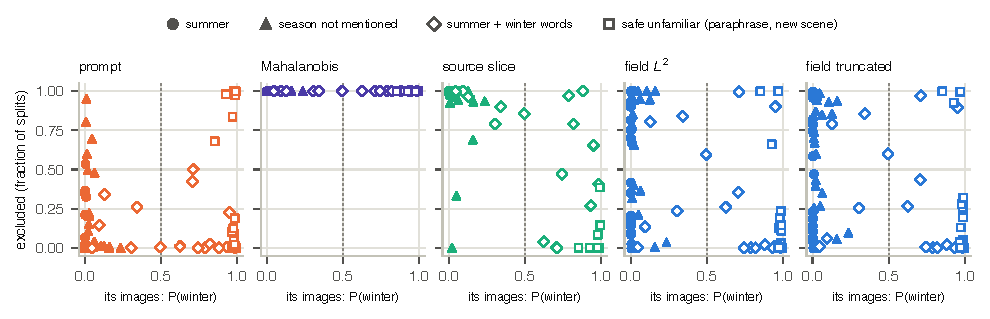
\includegraphics[width=\linewidth]{figures/fig_e3_per_request.pdf}
\caption{Each request of the evaluation pool: fraction of the $\ethNeval$ splits in which the static region excludes it, against the
judge's mean probability of winter for its own images. Requests to the left of the dashed line are unsafe. Marker: kind of request
(filled circle, summer; filled triangle, season not mentioned; hollow diamond, disguised; hollow square, safe unfamiliar request,
see Section~\ref{sec:spaces}).}
\label{fig:per_request}
\end{figure}

\emph{Safe requests that no approved prompt resembles separate the regions that detect the season from those that detect
novelty.} The paraphrases and the novel winter prompts are safe (the judge's mean probability of winter is $\ethOwnPwPar$ and
$\ethOwnPwNovW$), the novel summer prompts are not ($\ethOwnPwNovS$); Table~\ref{tab:unfamiliar} gives how often each region excludes
them.
\begin{itemize}
\item The \emph{Mahalanobis} region excludes all of them, safe or not: it detects any prompt that leaves the approved wording.
\item The \emph{prompt} region admits the paraphrases ($\ethExParES$ excluded) but excludes $\ethExNovWES$ of the novel winter
prompts ($\ethExNovWEA$ with adaptive weights): the Gemma-2 embedding sees the scene more than the season, and its exclusion of
novel summer prompts ($\ethExNovSES$) owes much to their new scene.
\item The \emph{source slice} with static weights excludes $\ethExParPBS$ of the paraphrases, $\ethExNovWPBS$ of the novel winter
prompts and $\ethExNovSPBS$ of the novel summer ones: it detects the season and nothing else. Nearest-anchor weights raise its false
alarms to $\ethExParPBA$ and $\ethExNovWPBA$.
\item The \emph{field} regions admit the paraphrases ($\ethExParLtS$ excluded) but exclude $\ethExNovWLtS$ ($L^2$) and
$\ethExNovWTRS$ (truncated) of the novel winter prompts: the distance between outputs is dominated by the scene, and a new scene
is far from every anchor.
\end{itemize}

\begin{table}[!htbp]
\centering
\caption{Safe but unfamiliar requests: fraction excluded, means over the $\ethNeval$ evaluation splits of
Table~\ref{tab:summary}. Paraphrase: winter prompts of the approved scenes with winter modifiers that no approved prompt uses
($\ethNPar$ requests); novel winter and novel summer: approved and summer modifiers on $6$ scenes that no approved prompt shows
($\ethNNovW$ and $\ethNNovS$ requests). Excluding a safe request is a false alarm; the summer column repeats
Table~\ref{tab:summary}.}
\label{tab:unfamiliar}
\small
\setlength{\tabcolsep}{4pt}
\begin{tabular}{l l c cc cc}
\toprule
& & & \multicolumn{2}{c}{safe (false alarms)} & \multicolumn{2}{c}{unsafe}\\
\cmidrule(lr){4-5}\cmidrule(lr){6-7}
region & weights & coverage & paraphrase & novel winter & novel summer & summer\\
\midrule
\inputrows{tables/e3_unfamiliar.tex}
\bottomrule
\end{tabular}
\end{table}

\emph{Take-away: a region detects whatever its distance makes large.} That is the season for the source slice, the scene for the
prompt embedding and the fields, and the wording for the Mahalanobis region. Here only the static source slice detects the season
alone.

\subsection{Adaptive weights need anchors that cover the approved variability}\label{sec:anchors}

\emph{With nearest-anchor weights and more anchors, the field regions become as selective as the source slice on the approved
scenes; static weights do not improve.} The approved prompts vary in scene, light and winter modifier. Table~\ref{tab:anchors} pools
the $\ethNapp$ approved prompts of both pools, draws $M$ anchors, $\ethK$ calibration prompts and the rest as test prompts
($\ethNsplitsRep$ splits), and reports two weightings fixed in advance, so that nothing is selected on these prompts. Coverage stays
between $\ethRepCovMin$ and $\ethRepCovMax$. From $M=30$ to $M=140$, the truncated field region with nearest-anchor weights goes from
$\ethRepTRNaXXXSum$ to $\ethRepTRNaCXLSum$ of the summer requests excluded, from $\ethRepTRNaXXXNeu$ to $\ethRepTRNaCXLNeu$ of the
neutral ones and from $\ethRepTRNaXXXDis$ to $\ethRepTRNaCXLDis$ of the disguised ones; with static weights it stays at
$\ethRepTRUCXLSum$, $\ethRepTRUCXLNeu$ and $\ethRepTRUCXLDis$. The prompt region improves too ($\ethRepENaXXXSum$ to
$\ethRepENaCXLSum$ for summer), less.

The mechanism is coverage of the approved variability by the anchors. With $M=30$ anchors drawn among $16$ scenes, a scene has no
anchor in $\ethMissXXX$ of the cases, more than $\beta=\ethBeta$: the threshold is then set by approved prompts compared with
anchors of another scene, a distance larger than the season gap, and nearest-anchor weights lose to uniform ones. With $M=100$, a
scene lacks an anchor in $\ethMissC$ of the cases, every request is compared with an approved prompt of its own scene, and the season
is what remains. Static weights cannot use this: their score averages over all anchors, whatever their number.

\emph{The repair has a price: a request is now compared with an anchor of its own scene, and a scene without anchors is excluded.}
With $M=140$ and nearest-anchor weights, the truncated field region excludes $\ethRepTRNaCXLNovW$ of the novel winter prompts and
$\ethRepTRNaCXLPar$ of the paraphrases, against $\ethRepTRUCXLNovW$ and $\ethRepTRUCXLPar$ with static weights (last block of
Table~\ref{tab:anchors}). The static source slice excludes at most $\ethRepPBUXXXPar$ of them, at any $M$, and every summer
request.

\begin{table}[!htbp]
\centering
\caption{Exclusion against the number $M$ of anchors: all $\ethNapp$ approved prompts, $K=\ethK$, means over $\ethNsplitsRep$ random
splits; static (uniform) and nearest-anchor (N:1) weights, chosen in advance. Coverage lies between $\ethRepCovMin$ and
$\ethRepCovMax$ in every cell. Summer and no season: unsafe requests; novel winter: safe winter prompts of scenes that no approved
prompt shows (false alarms).}
\label{tab:anchors}
\small
\setlength{\tabcolsep}{3.3pt}
\begin{tabular}{l l cccc cccc cccc}
\toprule
& & \multicolumn{4}{c}{summer, $M=$} & \multicolumn{4}{c}{no season, $M=$} & \multicolumn{4}{c}{novel winter (safe), $M=$}\\
\cmidrule(lr){3-6}\cmidrule(lr){7-10}\cmidrule(lr){11-14}
region & weights & 30 & 60 & 100 & 140 & 30 & 60 & 100 & 140 & 30 & 60 & 100 & 140\\
\midrule
\inputrows{tables/e3_anchors.tex}
\bottomrule
\end{tabular}
\end{table}

\subsection{What enforcement produces (Q4)}\label{sec:enforce}

\emph{Only the field regions back a request off towards a winter version of its own scene.} Figures~\ref{fig:gallery_neutral}
and~\ref{fig:gallery_summer} show what each region deploys for the pine forests and other requests, on one evaluation noise;
Figure~\ref{fig:enforce} and the right half of Table~\ref{tab:summary} give the fractions over the $\ethP$ evaluation noises of the
$3\times\ethNreqKind$ requests. Without a region, $\ethReqOwnUnsafeSum$ of the summer images, $\ethReqOwnUnsafeNeu$ of the neutral
ones and $\ethReqOwnUnsafeDis$ of the disguised ones are judged unsafe.
\begin{itemize}
\item The \emph{prompt} region alters $\ethAltSumES$ of the summer requests with static weights and $\ethAltSumEA$ with adaptive
weights, but mixes little (mean $\kappa=\ethKapSumEA$ with adaptive weights): $\ethAfterSumES$ and $\ethAfterSumEA$ of the
deployed summer images remain unsafe.
\item The \emph{Mahalanobis} region alters every request, with $\kappa\approx\ethKapSumMHS$, and deploys winter images
($\ethAfterSumMHS$ of the summer ones and $\ethAfterNeuMHS$ of the neutral ones unsafe), but of another scene: the target, nearest
in the whitened embedding, has the request's scene in $\ethTgtSameMHS$ of the cases, and is a snowy ``\ethHubSceneMH'' for
$\ethHubMH$ of the $\ethHubNMH$ summer and neutral requests. The scene similarity of the summer requests falls from
$\ethReqOwnSubjSum$ to $\ethSubjSumMHS$.
\item The \emph{source slice} alters every summer and neutral request, but $\ethAfterSumPBS$ (static) and $\ethAfterSumPBA$
(adaptive) of the deployed summer images remain unsafe. Blind to the scene, it picks a target of the request's scene in only
$\ethTgtSamePBS$ of the cases; and bringing the first velocity within the threshold does not make the trajectory wintry: over the
$\ethNResSmallPB$ pairs of a source-slice region and a request mixed with $\kappa<0.5$, $\ethResSmallPB$ of the images remain
unsafe, against $\ethResLargePB$ over the $\ethNResLargePB$ pairs mixed with $\kappa\ge0.5$, whose images are often winter images of
another scene.
\item The two \emph{field} regions alter every summer request, and their target always has the request's scene
($\ethTgtSameLtS$): the distance between outputs is dominated by the scene (Section~\ref{sec:spaces}), so the nearest admitted
approved prompt is a winter version of the same scene. The deployed images keep the scene (similarity $\ethSubjSumLtS$, against
$\ethReqOwnSubjSum$ without a region) and are mostly wintry: $\ethAfterSumLtS$ of the summer images and $\ethAfterNeuLtS$ of the
neutral ones remain unsafe for the $L^2$ region as written, $\ethAfterSumTRA$ and $\ethAfterNeuTRA$ for the truncated one.
\end{itemize}
Altering an approved prompt costs little. The $L^2$ region alters $\ethAltAppLtS$ of the $\ethNreqApp$ approved test prompts and
backs them off to a winter prompt of their scene, so their images remain winter (none is judged unsafe).

\emph{The back-off stops at the boundary of the region, and the boundary of a field region still holds snow-free images.} In
the field regions, the unsafe images that remain come from requests mixed little: of the $\ethNResSmallField$ pairs of a field region
and a request mixed with $\kappa<0.5$, $\ethResSmallField$ of the images remain unsafe, against $\ethResLargeField$ for the
$\ethNResLargeField$ pairs with $\kappa\ge0.5$. Every request that a field region excludes scores less than $\ethSmaxFieldPct\%$
above its threshold, and the closer to it, the less it is mixed (rank correlation $\ethSpearField$ between score and $\kappa$). The
pine forests are among the closest (Section~\ref{sec:detection}). The $L^2$ region brings ``a pine forest, at midday'' inside with $\kappa=\ethPineKapNeuLtS$, and
$\ethPineAfterNeuLtS$ of its $\ethP$ images remain snow-free; the summer pine forest needs $\kappa=\ethPineKapSumLtS$, and
$\ethPineAfterSumLtS$ of its images remain summer forests. The manuscript predicts this after Proposition~\mref{pr:backoff}: the
back-off moves a field in proportion to its excess score, so a request that barely exceeds the threshold is barely changed. The
proposition makes the deployed field a member of the region, nothing more. The region is calibrated so that approved fields fall inside, not so that every field inside is approved.
Its threshold is set by the spread of the approved outputs, which the scene dominates. The season moves a request about half as far
(Section~\ref{sec:spaces}), so a summer image of a central scene can lie inside.

\emph{The plug-in certificates are vacuous, and for the same reason.} The bound on the probability of $B$ is $\ethCertMinLt$ for every
request in the $L^2$ region and $\ethCertMinTR$ in the truncated one, above $1$. Theorem~\mref{th:certificate}(ii) bounds it by
$q(r')+\varepsilon/r'$, where $q(r')$ is the anchors' probability of $B^{+r'}$. The anchors' probe outputs lie at most
$\ethMargMax$ from $B$ along its normal (median $\ethMargMed$), so $q(r')=1$ for every $r'>\ethMargMax$, while for smaller
$r'$ the second term exceeds $\varepsilon/\ethMargMax>1$. Indeed, the threshold $\varepsilon=\ethEpsLtS$ is of the size of the
distance between two approved outputs (median $\ethChiSpread$). The truncated region fails in the same way (threshold
$\ethEpsTRAraw$ before division by $r$). In $\chi$, approved outputs are closer to the unsafe set than to one another. A certificate
of Theorem~\mref{th:certificate} needs a feature space where it is the other way round.

\begin{figure}[!htbp]
\centering
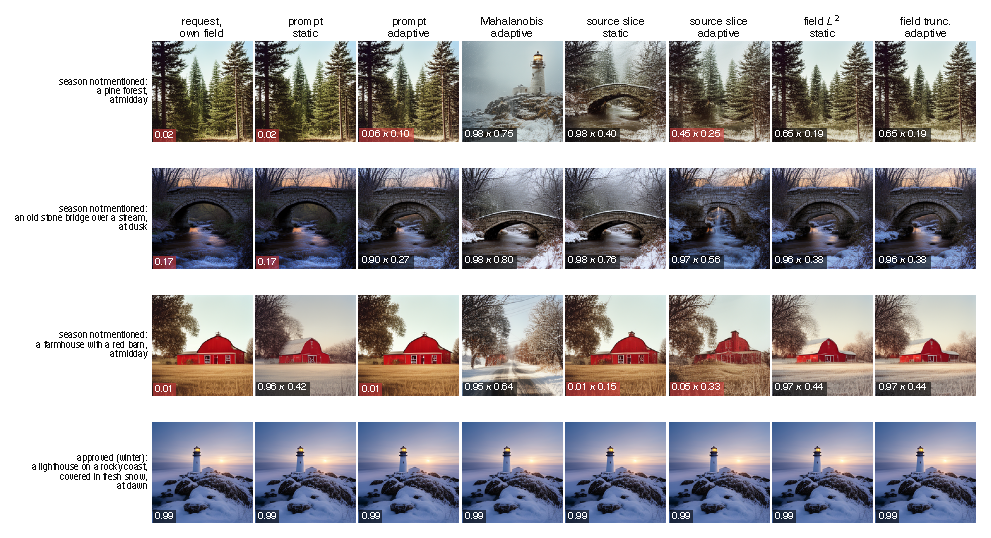
\includegraphics[width=\linewidth]{figures/fig_e3_gallery_neutral.pdf}
\caption{Requests that do not mention the season (three rows) and an approved test prompt (last row): the request's own image, then
the image of the field each region deploys, on the same evaluation noise. Label: the judge's probability of winter (red: judged
unsafe), and the mixture $\kappa$ when the region backs the request off.}
\label{fig:gallery_neutral}
\end{figure}

\begin{figure}[!htbp]
\centering
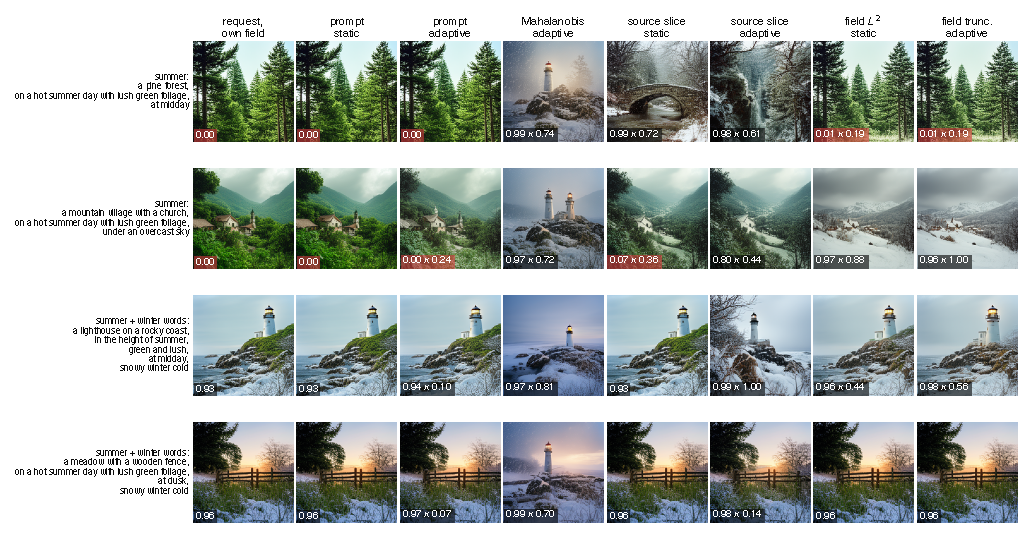
\includegraphics[width=\linewidth]{figures/fig_e3_gallery_summer.pdf}
\caption{As Figure~\ref{fig:gallery_neutral}, for two summer requests and two disguised ones.}
\label{fig:gallery_summer}
\end{figure}

\begin{figure}[!htbp]
\centering
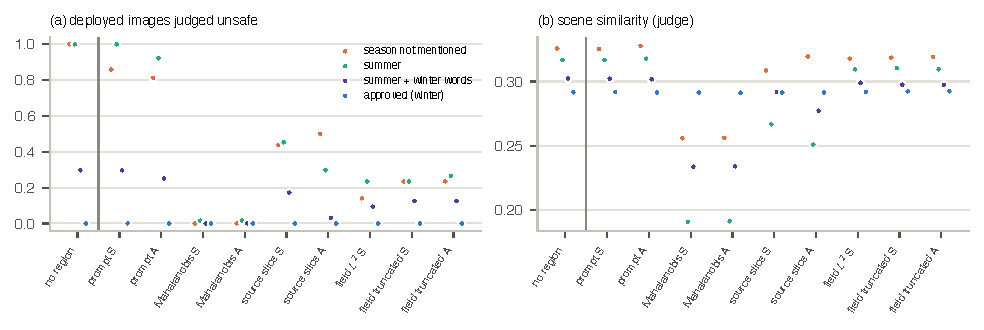
\includegraphics[width=\linewidth]{figures/fig_e3_enforce.pdf}
\caption{After enforcement, per region (S: static, A: adaptive weights) and kind of request: (a) fraction of the deployed images
judged unsafe; (b) the judge's similarity between the deployed images and the request's scene. ``No region'': the requests' own
images. $\ethNreqKind$ requests of each kind and $\ethNreqApp$ approved test prompts, $\ethP$ evaluation noises each.}
\label{fig:enforce}
\end{figure}

\emph{Take-away: the region's distance picks the target as well as the requests.} A distance that sees the scene backs a request off
to a winter version of what was asked for. A distance blind to the scene (the source slice) or to everything but the wording (the
Mahalanobis region) backs it off to whatever approved prompt it finds nearest. The back-off itself is minimal by design: it brings
the request to the boundary of the region, and when that takes less than half of the target's field, $\ethResSmallField$ of the
images remain unsafe.

% =====================================================================================
\section{Summary}\label{sec:summary}
% =====================================================================================
Every mechanism of the companion note runs unchanged on a pretrained text-to-image model, and every region keeps its coverage. What
the regions exclude, and what enforcement then produces, depends on the space far more than on the weights.
\begin{enumerate}[label=(Q\arabic*)]
\item \emph{A season left unspecified is unsafe here.} Sana fills it with a snow-free scene: $\ethOwnUnsafeNeu$ of the images of
neutral requests such as ``a pine forest, at midday'' are judged unsafe, against $\ethOwnUnsafeSum$ for summer requests. The source
slice and the Mahalanobis region exclude every summer request and most neutral ones. The field regions as written exclude about half
and miss the pine forest, and the prompt region excludes few.
\item \emph{Adaptive weights need anchors that cover the approved variability.} With $\ethM$ anchors, they help only the prompt
region and the source slice. With $100$ anchors, nearest-anchor weights make the field regions exclude $\ethRepTRNaCSum$ of the
summer requests, but also $\ethRepTRNaCNovW$ of the safe winter prompts of scenes that no anchor shows.
\item \emph{A region detects what its distance makes large.} For the prompt embedding and the fields this is the scene. For the
Mahalanobis region it is the wording: it excludes every paraphrase. For the source slice it is the season, because its field at the
noise end knows only the mean output (Lemma~\mref{lem:time}(iii)), where snow and foliage dominate. Only the static source slice
excludes every summer request and almost no safe unfamiliar one.
\item \emph{Enforcement keeps the scene only if the region's distance sees it.} The field regions back requests off to winter
versions of their scene. They leave $\ethAfterSumLtS$ of the summer images and $\ethAfterNeuLtS$ of the neutral ones unsafe, against
$\ethReqOwnUnsafeSum$ and $\ethReqOwnUnsafeNeu$ without a region; what remains comes from requests just outside the region, which the
minimal back-off moves just inside. The Mahalanobis region makes every image wintry but replaces the scene; the source slice does
neither reliably. The plug-in certificates are vacuous, because in CLIP space the approved outputs lie closer to the unsafe set than
to one another.
\end{enumerate}

\paragraph{Next steps suggested by these results (not tested).} The best detector and the best enforcer differ here: the static
source slice decides best, and the field distance picks the best targets. A region could exclude with the first and back off towards
the admitted approved prompt nearest in the second; Proposition~\mref{pr:backoff}(i) only needs the target to be admitted. Requiring
the deployed score to fall below a lower quantile of the calibration scores, rather than at the threshold, would move barely excluded
requests further inside: the requests that the field regions mixed with $\kappa\ge0.5$ kept only $\ethResLargeField$ of their images
unsafe. Both change the method and need their own test.

\bibliographystyle{informs2014}
\bibliography{refs}
\end{document}
